% id: 93-178
% book: 개념원리 기하 · 10 직선과 평면의 수직
% section: 연습문제 실력 UP
% figure: crop:fig-93-178.png
% answer: $\sqrt{6}$
% answer_source: 답지
% variant_level: 0 (원본 전사)
% 이 파일은 build.mjs 가 items.json 에서 만든다. 고칠 때는 items.json 을 고친다.
\smash{\raisebox{1.5mm}{\dmkichul{개념원리 기하 93쪽 178번}}}
\noindent\begin{minipage}[t]{0.58\linewidth}\vspace{0pt}\raggedright 오른쪽 그림과 같이 한 모서리의 길이가 $6$인 정육면체에서 두 점 $\pt{P}$, $\pt{Q}$는 각각 $\seg{BD}$, $\seg{AG}$ 위에 있고, $\seg{PQ}$는 $\seg{BD}$와 $\seg{AG}$에 각각 수직이다. 이때 선분~$\pt{PQ}$의 길이를 구하시오.\end{minipage}\hfill\begin{minipage}[t]{0.4\linewidth}\vspace{0pt}\centering \setlength{\dmfigw}{70.7pt}\ifdim\dmfigw>\linewidth\setlength{\dmfigw}{\linewidth}\fi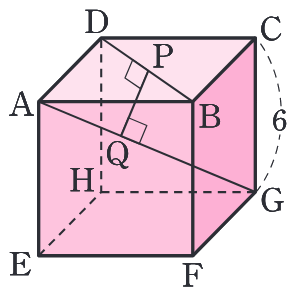
\includegraphics[width=\dmfigw]{figures/fig-93-178.png}\end{minipage}\par
